\documentclass{beamer}
\usetheme{CambridgeUS}
\usecolortheme{dolphin}

\usepackage[citestyle=authortitle-icomp]{biblatex}
\usepackage{nth}
\usepackage{pgfpages}
\usepackage{relsize}
\usepackage[group-separator={,},group-minimum-digits=4]{siunitx}
\usepackage{tikz}
\usepackage{todonotes}

% \setbeameroption{show notes on second screen=right}

\presetkeys{todonotes}{inline}{}

\graphicspath{{../../figures/small/}}

\setbeamertemplate{caption}{\raggedright\insertcaption\par}
\setbeamerfont{caption}{size=\scriptsize}
\setbeamertemplate{navigation symbols}{}

\newcommand{\Beta}{B}

\newcommand{\mathA}{\mathcal{A}}
\newcommand{\mathB}{\mathcal{B}}
\newcommand{\mathC}{\mathcal{C}}
\newcommand{\mathG}{\mathcal{G}}
\newcommand{\mathP}{\mathcal{P}}

\title[Bayesian Income Inference]{A Bayesian Approach to Income Inference \\ in a Communication Network}

\author[Fixman et.\ al]{%
	Martin~Fixman\inst{1}\inst{2}\and
	Ariel~Berenstein\inst{1}\and
	Jorge~Brea\inst{1}\and \\
	Martin~Minnoni\inst{1} \and
	Carlos~Sarraute\inst{1}
}

\institute[FCEyN UBA \and Grandata]{%
	\inst{1}Grandata Labs, Bartolome Cruz 1818, Vicente Lopez, Argentina \\
	\inst{2}Universidad de Buenos Aires, Argentina \\
	\texttt{ \{mfixman, ariel, jorge, martin, charles\}@grandata.com }
}

\date[Workshop AGRANDA]{Workshop AGRANDA \\ September 7, 2016}

\addbibresource{../../Asonam2016/bibliography/sna.bib}{}

\begin{document}

\begin{frame}
	\titlepage{}
\end{frame}

\section{Introduction}
\subsection{Introduction}

\begin{frame}{Introduction}
\note{%
	In recent years, we have witnessed an exponential growth in the capacity to gather, store and manipulate massive amounts of data across a broad spectrum of disciplines.

	Mobile phone datasets provide a very rich view into the social interactions and the physical movements of large segments of a population.

	In Grandata, we work with the datasets a big telco and a big bank in Mexico to infer the socioeconomic data of their users using data mining approaches.
}

	In recent years, we have witnessed an exponential growth in the capacity to gather, store and manipulate massive amounts of data across a broad spectrum of disciplines.

	Mobile phone datasets provide a very rich view into the social interactions and the physical movements of large segments of a population.
\end{frame}

\subsection{Understanding the Social Graph}

\begin{frame}{Understanding the Social Graph}
\note{%
	The voice calls and text messages exchanged between people, together with the call locations (recorded through cell tower usages), allow us to construct a rich social graph which can give us interesting insights on the users' social fabric, detailing not only particular social relationships and traits, but also regular patterns of behavior both in space and time, such as their daily and weekly mobility patterns
}

\begin{equation*}
	G = \left< \text{users}, \text{calls} \right>
\end{equation*}

We use the \textbf{Social Graph} to understand users' behaviour.\footcite{gonzalez2008understanding}\footcite{ponieman2013human}\footcite{sarraute2015city}

\begin{center}
\tikzstyle{att} = [circle, draw, fill=black!25, minimum size=10pt]
\tikzstyle{edge} = [draw, thick, >=latex]

\begin{tikzpicture}
	\node[att] (0) at (-2, 0) {};
	\node[att] (1) at (0, 0) {};
	\node[att] (2) at (0, -2) {};
	\node[att] (3) at (-2, -2) {};
	\node[att] (4) at (-1, -1) {};
	\node[att] (5) at (-3, -1) {};
	\path[edge, ->] (0) -- (1);
	\path[edge, ->] (1) -- (2);
	\path[edge, ->] (2) -- (3);
	\path[edge, <->] (3) -- (0);
	\path[edge, ->] (0) -- (4);
	\path[edge, <->] (4) -- (2);
	\path[edge, ->] (4) -- (3);
	\path[edge, <->] (5) -- (0);
	\path[edge, ->] (5) -- (3);

	\node[att] (a) at (1, 0) {};
	\node[att] (e) at (1, -1.5) {};
	\path[edge, <->] (1) -- (a);
	\path[edge, <-] (1) -- (e);
	\path[edge, ->] (2) edge [bend right = 30] (e);

	\path[edge, ->] (e) -- (a);
\end{tikzpicture}

\end{center}

\end{frame}

\begin{frame}
\note{%
	Economic factors are also believed to have a determining role in both the social network's structure and dynamics. In particular, individuals have a tendency to establish links with others of a similar socioeconomic background, which results in social stratification.

	(pause)

	In this work, we leverage the socioeconomic homophily present in the cellular phone network to generate inferences of socioeconomic status in the communication graph. To this aim we use two data sources:

	\begin{enumerate}
		\item The Call Detail Records from the operator, which allows us to construct a social graph.
		\item Reported income from a subset of clients obtained from a large bank.
	\end{enumerate}

	This allows us to take advantage of both the individual users' features and the topology of the phone network.
}

\begin{itemize}
	\item Economic factors determine the structure of the Social Network.
	\begin{itemize}
		\item People tend to call other people of similar socioeconomic status.\footcite{leo2015socioeconomic}
	\end{itemize}

	\pause{}

	\item Two separate data sources.

	\begin{enumerate}
		\item The Call Detail Records from the operator.
		\item Reported income from a subset of clients obtained from a large bank.
	\end{enumerate}

	\item We use this data to \textit{infer} the socioeconomic status of users which aren't in the bank subset.
\end{itemize}

\end{frame}

\section{Data Sources}
\subsection{Bank Data Source}

\begin{frame}{Bank Data Source}
\note{%
	For this study, we got access the account balances of over 10 million clients of a mexican bank for a period of 6 months, denoted \( \mathB \). We also have some demografic information of a subset \( \mathA \subseteq \mathB \), including the users' age.
}

\begin{itemize}
	\item Income data for \num{10000000} clients.
	\item Demographic data (age and gender) for a smaller subset.
\end{itemize}

\begin{figure}[h]
	\begin{center}
		{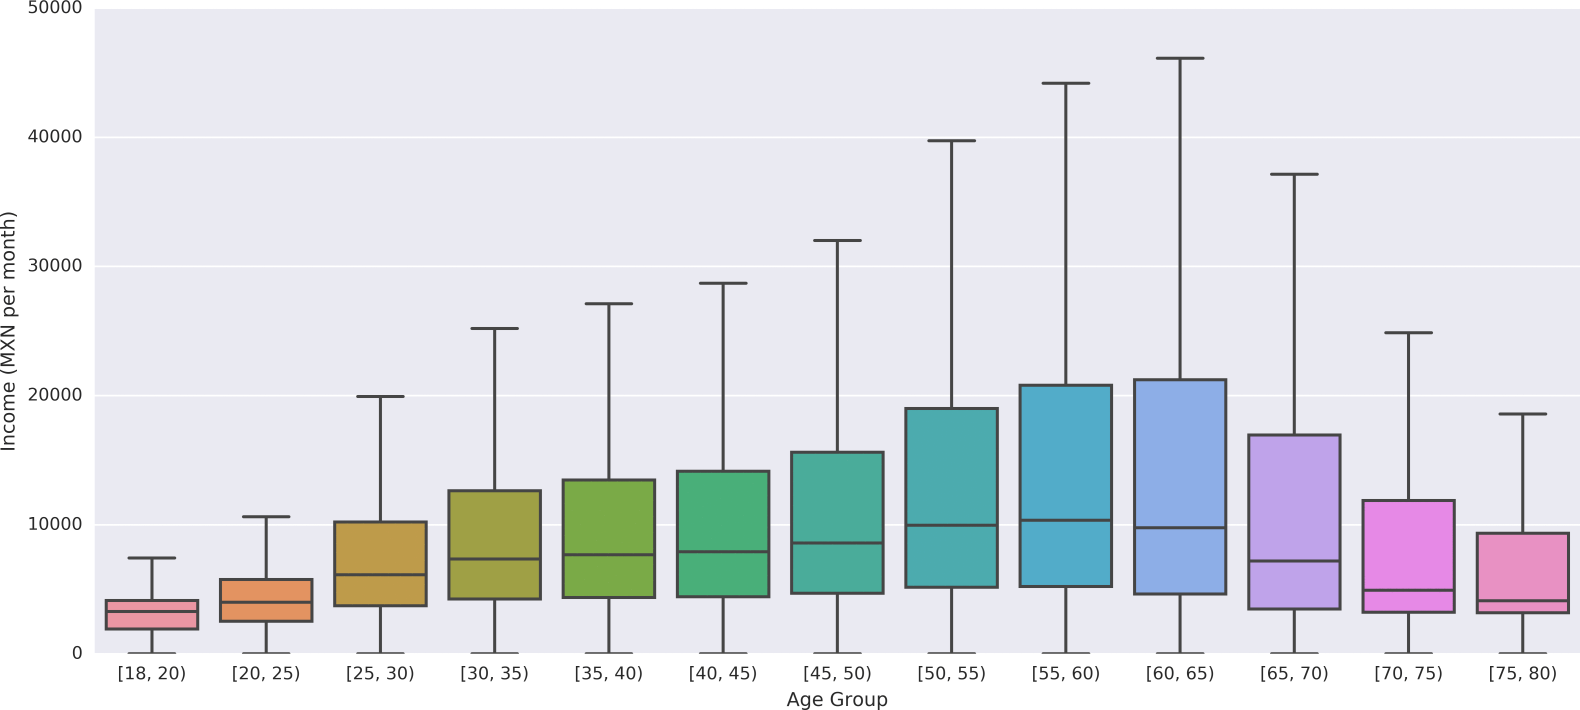
\includegraphics[width=\columnwidth]
				{income_age_boxplot4_wide.png}
		}\label{income_age_boxplot}
	\end{center}
\end{figure}
\end{frame}

\subsection{Mobile Phone Data Source}

\begin{frame}{Mobile Phone Data Source}
\note{%
	The main dataset for this study consists of a set \( \mathP \) of \textit{Call Detail Records} composed of voice calls and text messages from a Mexican telco for a 3 month period. Since we only have complete data for users of the telco, we work on set of calls \( \mathG_N \) between these users.

	The data in \( \mathB \) contains the self-reported phone numbers of the bank user, which the bank hashes with the same function as the telco uses for the CDRs. Thanks to this fact, we can correlate telco users with bank users to create the \textbf{social graph} \( G \).
	\[
		G = \mathP \bowtie_{\operatorname{originUser}} \mathB \bowtie_{\operatorname{targetUser}} \mathB
	\]

	This graph has a total of \num{2027554} nodes with \num{5044976} edges, which represent \num{29599762} calls and \num{5476783} text messages.
}

\begin{itemize}
	\item Set \( \mathG_N \) of \textit{Call Detail Records}
	\begin{itemize}
		\item A total of \num{2027554} users.
		\item \num{29599762} calls between \num{5044976} pairs.
	\end{itemize}
	\item Self-reported phone number \( \mathB \) of the bank account.
	\begin{itemize}
		\item Hashed with the same function as the phone numbers in \( \mathG_N \).
	\end{itemize}
	\item We join this dataset with the bank to create the \textbf{Social Graph} \( G \).

	\[
		G = \mathP \bowtie_{\operatorname{originUser}} \mathB \bowtie_{\operatorname{targetUser}} \mathB
	\]
\end{itemize}

\end{frame}

\section{Inference Methodology}
\subsection{Income Homophily}

\begin{frame}{Inference Methodology}
\note{%
	The main part of this work is based on the observed homophily between income levels of the participants in a phone call. That is, if person \emph{X} calls person \emph{Y}, then there's a high change that \emph{X} and \emph{Y} have similar incomes.

	We can observe this homophily in the source data by measuting \textbf{Spearman's Rank Correlation} to test the statistical dependence of sets \emph{X} and \emph{Y}. This correlation uses the rank of the variable instead of the value, so it's independent in differences in relative wealth between social groups.

	\[
		r_s = \mathlarger{\rho}_{\operatorname{rank}(X) \operatorname{rank}(Y)} = \frac{\operatorname{cov} \left( \operatorname{rank}(x), \operatorname{rank}(y) \right)}{\sigma_{\operatorname{rank}(X)} \sigma_{\operatorname{rank}(Y)}}
	\]

	This formula gives us a correlation coefficient of \( \mathbf{r_s = 0.474} \). Compared to a randomized null hypothesis, where links between users are selected randomly disregarding income data, we have a p-value of \( p < 10^{-6} \).
}

\begin{itemize}
	\item We assume that there is homophily between participants in a phone call.
	\begin{itemize}
		\item If user \textit{X} cals user \textit{Y}, then \textit{X} and \textit{Y} probably have similar incomes.
	\end{itemize}
	\item We can measure this calculating the \textbf{Spearman's Rank Correlation} of the data.
\end{itemize}

\[
	r_s = \mathlarger{\rho}_{\operatorname{rank}(X) \operatorname{rank}(Y)} = \frac{\operatorname{cov} \left( \operatorname{rank}(x), \operatorname{rank}(y) \right)}{\sigma_{\operatorname{rank}(X)} \sigma_{\operatorname{rank}(Y)}}
\]

\begin{itemize}
	\item Correlation coefficient is \( \mathbf{r_s = 0.474} \): there's a significant correlation.
\end{itemize}

\end{frame}

\begin{frame}
\note{%
	The income homophily can be easily seen when plotting the data.
}

\begin{figure}[h]
	\begin{center}
		{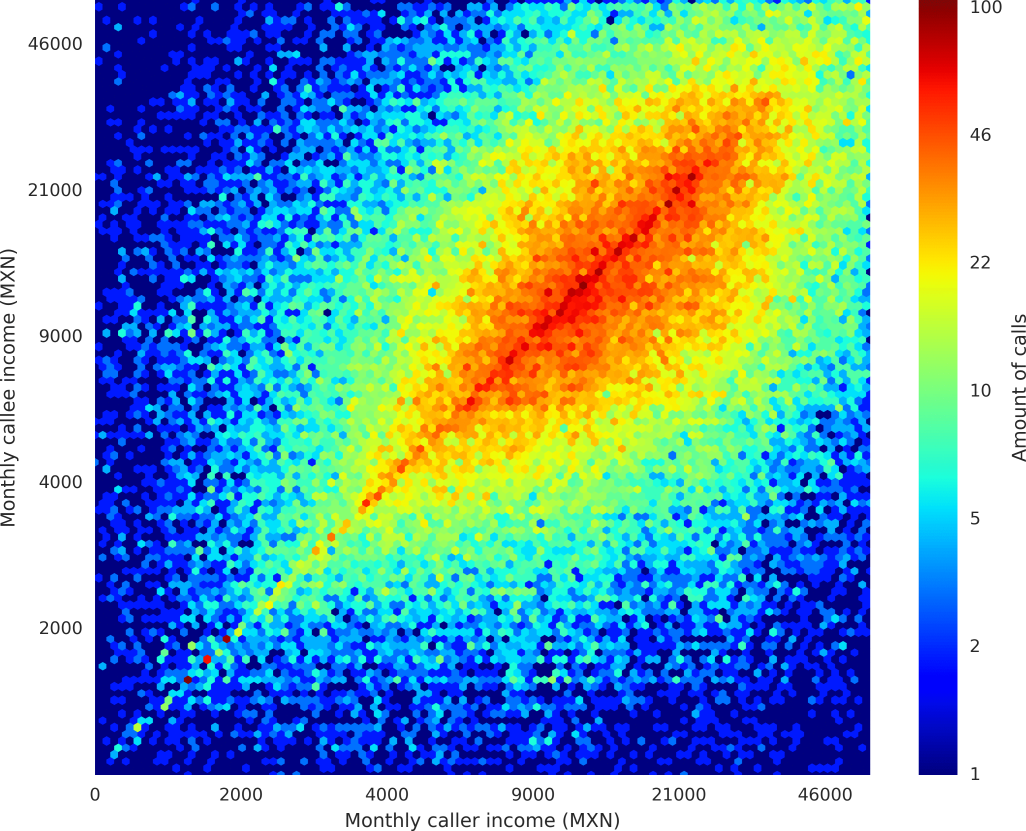
\includegraphics[height=0.8\textheight]
		{Homophily_income_origin_target_1.png}
		}\label{homophily_heatmap}
	\end{center}
	\caption{The income homophily can be easily seen when plotting the data.}
\end{figure}

\end{frame}

\subsection{Prediction Algorithm}
\begin{frame}{Prediction Algorithm}
\note{%
	We separate the users in our input into two disjoint groups, which have roughly the same amount of people in our dataset after removing outliers.

	\begin{description}
		\item[Poor People] have less than \num{3600}~MXN\footnote{3600~MXN = 343~USD = \num{5095}ARS} in their bank account.
		\item[Wealthy People] have more than \num{3600}~MXN.
	\end{description}

	According to our hypothesis, poor people should have more calls to other poorer people, while wealthy people should have a higher proportion of calls to wealthier ones.
}

\begin{itemize}
	\item Users are separated in two groups.
	\begin{description}
		\item[Low income] receive less than \num{3600}~MXN\footnote{3600~MXN = 343~USD = \num{5095}ARS} in their bank account per month.
		\item[High income] receive more than \num{3600}~MXN.
	\end{description}
	\item According to our hypothesis, if a person calls mostly users from one of the groups then its part of that group.
\end{itemize}
\end{frame}

\begin{frame}
\note{%
	The simpler method for inferring the category of each user with this data is \textbf{Majority Voting}, which gives each user the category for which the majority of its contacts belongs. This has an accuracy of 66\%, which is way better than the 50\% you get from random selection, but still can be improved.

	(pause)

	A better approach, presented by this paper, uses \textbf{Bayesian Inference} to solve this problem
}

\begin{itemize}
	\item<1-> \textbf{Random Selection} 50\%~accuracy.
	\item<1-> \textbf{Majority Voting} same category as the majority of its contacts. 66\%~accuracy.
	\item<2-> \textbf{Bayesian Inference} where we define a probability distribution for one category using a \textbf{Beta~Distribution}.
\end{itemize}

\end{frame}

\subsection{Bayesian Approach}
\begin{frame}{The Bayesian Approach}
\note{%
	A better approach, presented by this paper, uses \textbf{bayesian inference} to solve this problem. We can define, for each user \( j \) with \( \alpha^j \) calls to wealthy people and \( \beta^j \) calls to poor people, a \textbf{beta distribution} \( \beta^j ( x; \alpha^j, \beta^j ) \) which gives the probability distributions of belonging to one category.

	\( \alpha^j \) calls to wealthy users.

	\( \beta^j \) calls to poor users.

	\( B^j \left( x; \alpha^j, \beta^j \right) \) is the distribution of probabilities that the user \( j \) is wealthy.

	To make sure we take into account both the mean and the variance of the distribution, we take the \nth{5} percentile of the \textbf{cumulative distribution function} of the beta distribution for each user. We can see in this graph how the same ratio of wealthy to poor contacts could give a different value for the integral.

	(pause)

	We take some threshold \( \tau \), and define rich users as people where that value if higher than that threshold.
}

\begin{overlayarea}{\textwidth}{.3\textheight}
\begin{itemize}
		\item We define a \textbf{Beta~Distribution} with two parameters.
		\begin{itemize}
			\item \( \alpha^j \) calls to wealthy users.
			\item $ \beta^j $ calls to poor users.
		\end{itemize}
		\item \( B^j \left( x; \alpha^j, \beta^j \right) \) is the distribution of the probability that user $ j $ is wealthy.

\end{itemize}
\end{overlayarea}

\begin{overlayarea}{\textwidth}{.7\textheight}
	\alt<1>{%
		\begin{figure}
		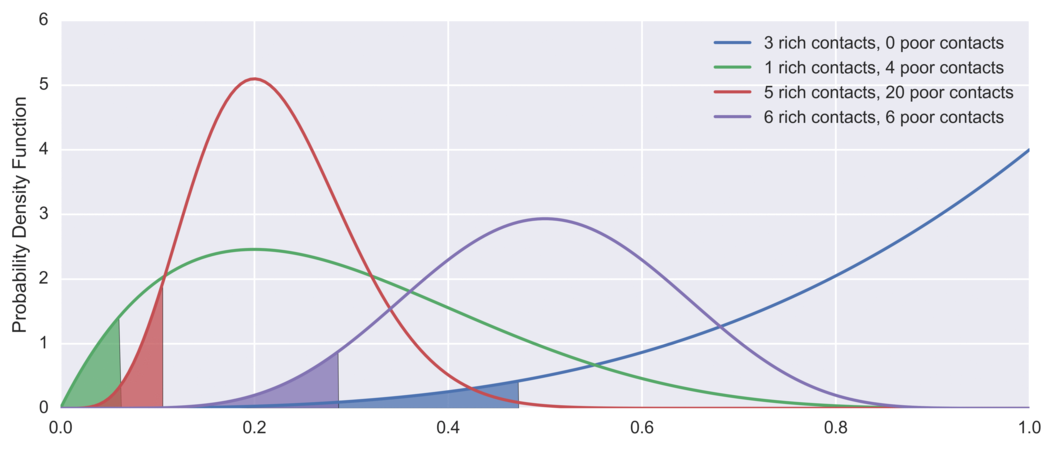
\includegraphics[height=.45\textheight]{Beta_example.png}
		\caption{Value of the 5th percentile for different neighbours' socioeconomic levels.}
		\end{figure}
	}{}

	\alt<2>{%
		\begin{itemize}
			\item We then take the \nth{5} percentile of the CDF for each user \( k_i \).
			\item A user is wealthy if \( k_i > \tau \) for some parameter \( \tau \).
		\end{itemize}
	}{}
\end{overlayarea}

\end{frame}

\section{Results}
\subsection{ROC Curve}
\begin{frame}[fragile]{Results}
\note{%
	\( \tau \) balances the precision and recall of each users' distribution.

	We can plot the True Positive Rate and the False Positive Rate of the distribution in a ROC Curve to select the most optimal \( \tau \).

	(pause)

	In our case, the optimal \( \tau \) is 0.4, which gives us an accuracy for predicting the wealth category of 71\%.
}
	\begin{overlayarea}{\textwidth}{2.5em}
		\alt<1>{%
			\begin{itemize}
				\item \( \tau \) balances the precision and recall of each users' distribution.
				\item This curve has an \textbf{AUC} of \num{0.74}.
			\end{itemize}
		}{}
		\alt<2->.
			\end{itemize}
		}{}
	\end{overlayarea}

	\begin{overlayarea}{\textwidth}{.9\textheight}
		\alt<1>{%
			\begin{figure}
				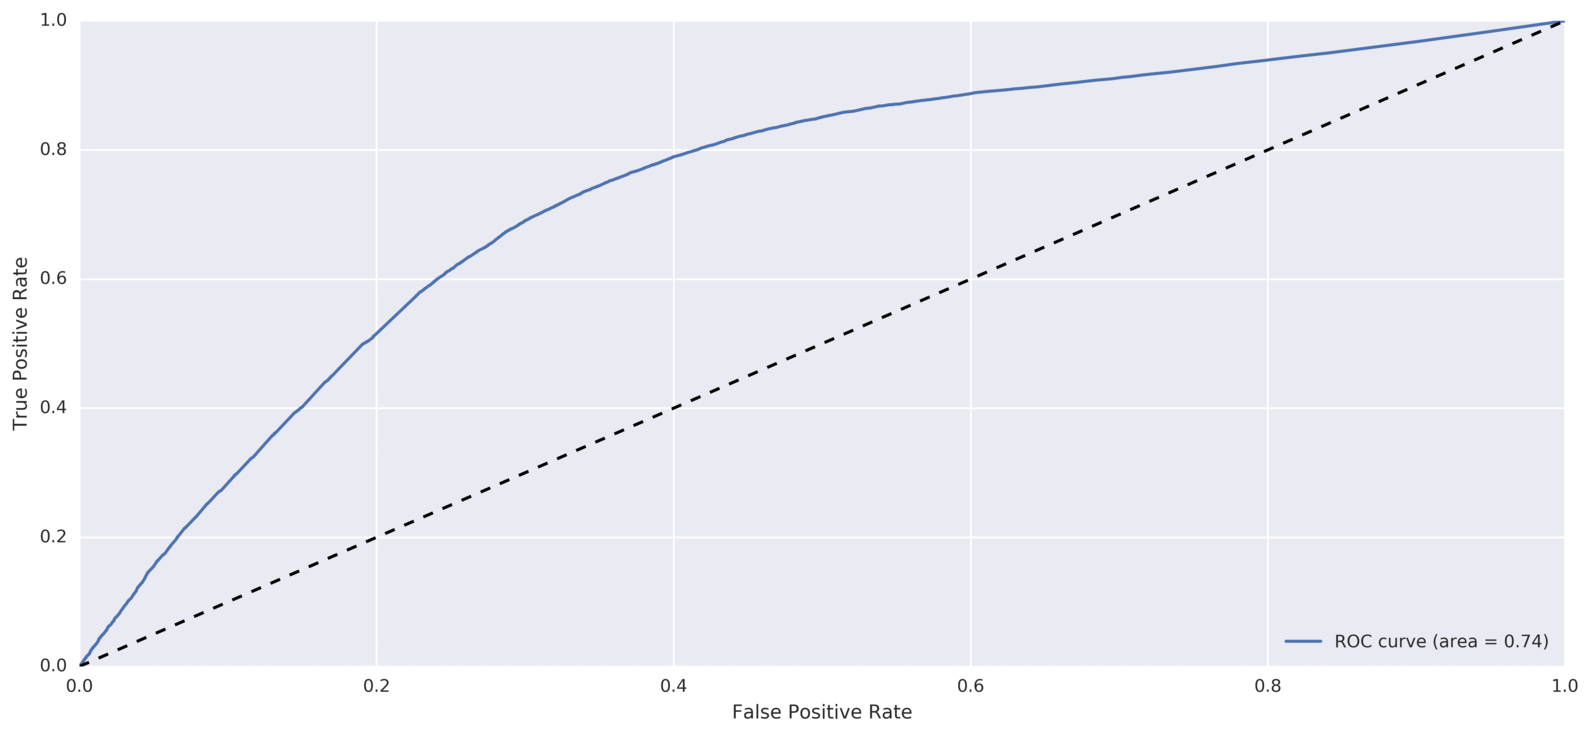
\includegraphics[width=\textwidth]{roc_curve_wide.png}
				\caption{ROC Curve with \textit{False Positive Rate} plotted against the \textit{True Positive Rate}}
			\end{figure}
		}{}
		\alt<2>{%
			\begin{figure}
				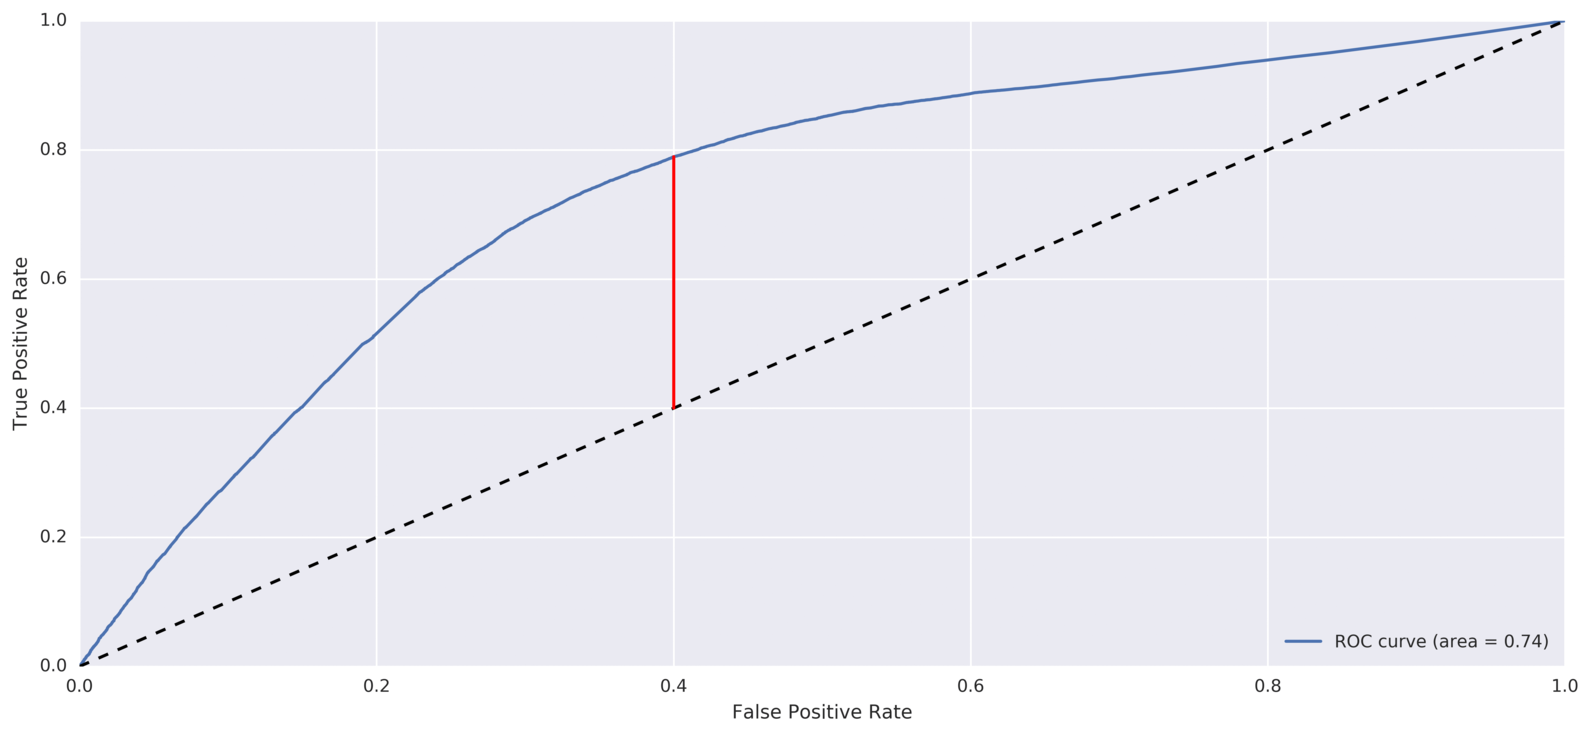
\includegraphics[width=\textwidth]{roc_curve_marked_wide.png}
				\caption{ROC Curve with \textit{False Positive Rate} plotted against the \textit{True Positive Rate}}
			\end{figure}
		}{}
		\alt<3>{%
			\begin{figure}
			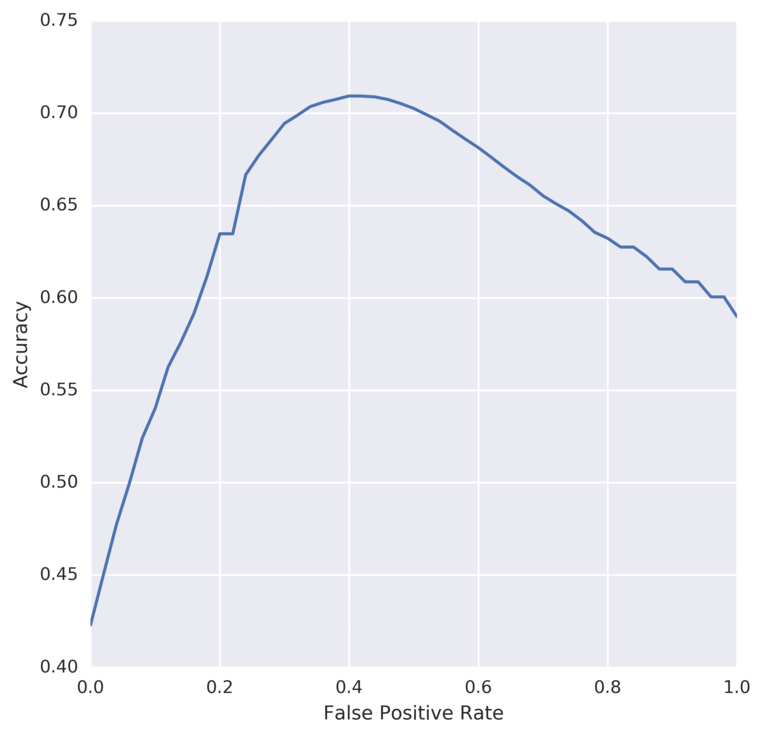
\includegraphics[width=\textwidth]
			{accuracy.png}
			\caption{Model accuracy plotted against False Positive Rate}
			\end{figure}
		}{}
	\end{overlayarea}
\end{frame}

\section{Future Work}
\subsection{Extension to Multiple Categories}

\begin{frame}{Extension to Multiple Categories}
\note{%
	There are several improvemente we can make to this algorithm. Our next line of work consists of separating the groups into more than 2 categories.

	In this case, we define 5 categories depending on a users' wealth.

	\begin{description}[leftmargin=!]
		\item[\(R_1\)] \num{1000}~MXN
		\item[\(R_2\)] \num{2500}~MXN to \num{7500}~MXN
		\item[\(R_3\)] \num{7500}~MXN to \num{20000}~MXN
		\item[\(R_4\)] \num{20000}~MXN to \num{50000}~MXN
		\item[\(R_5\)] More than \num{50000}~MXN
	\end{description}
}

5 categories to describe a users' wealth:

\begin{description}[leftmargin=!]
	\item[\(R_1\)] \num{1000}~MXN\footnote{\num{1000}~MXN = \num{53.79}~USD = \num{806.52} ARS} to \num{2500}~MXN\footnote{\num{2500}~MXN = \num{134.47}~USD = \num{2016.30}~ARS}
	\item[\(R_2\)] \num{2500}~MXN to \num{7500}~MXN\footnote{\num{7500}~MXN = \num{403.41}~USD = \num{6048.89}~ARS}
	\item[\(R_3\)] \num{7500}~MXN to \num{20000}~MXN\footnote{\num{20000}~MXN = \num{1075.75}~USD = \num{16130.37}~ARS}
	\item[\(R_4\)] \num{20000}~MXN to \num{50000}~MXN\footnote{\num{50000}~MXN = \num{2689.37}~USD = \num{40325.93}~ARS}
	\item[\(R_5\)] More than \num{50000}~MXN
\end{description}

\end{frame}

\begin{frame}
\note{%
	Instead of using a Beta Distribution for each user \( j \), we define a \textbf{Dirichlet distribution} for each category, taking \( \alpha^j_i \) as the number it has with users to the category \( i \).

	\[
		D^j \left( x_1, \ldots, x_5; \alpha^j_1, \ldots, \alpha^j_5 \right) = \frac{1}{\Beta(\alpha)} \prod^5_{i = 1}{x_i^{\alpha^j_i - 1}}
	\]

	The result of the distribution is 5 distributions for each user, which gives the probability of each user to belong to each category.
}

\begin{itemize}
	\item We use a \textbf{Dirichlet distribution} for each category.
	\begin{itemize}
		\item \( \alpha^j_i \) is the number of calls user $j$ has with users in category \( i \).
	\end{itemize}

	\[
		D^j \left( x_1, \ldots, x_5; \alpha^j_1, \ldots, \alpha^j_5 \right) = \frac{1}{\Beta(\alpha)} \prod^5_{i = 1}{x_i^{\alpha^j_i - 1}}
	\]

	\item 5 distinct distributions for each user.
	\item \( D^j \) is the probability distributions that user \( j \) is part of each category.
\end{itemize}
\end{frame}

\begin{frame}
\note{%
	We can create 5 new ROC Curves with this data, which have higher \textbf{Area Under the Curves} than the case with majority voting.
}
	\begin{figure}
		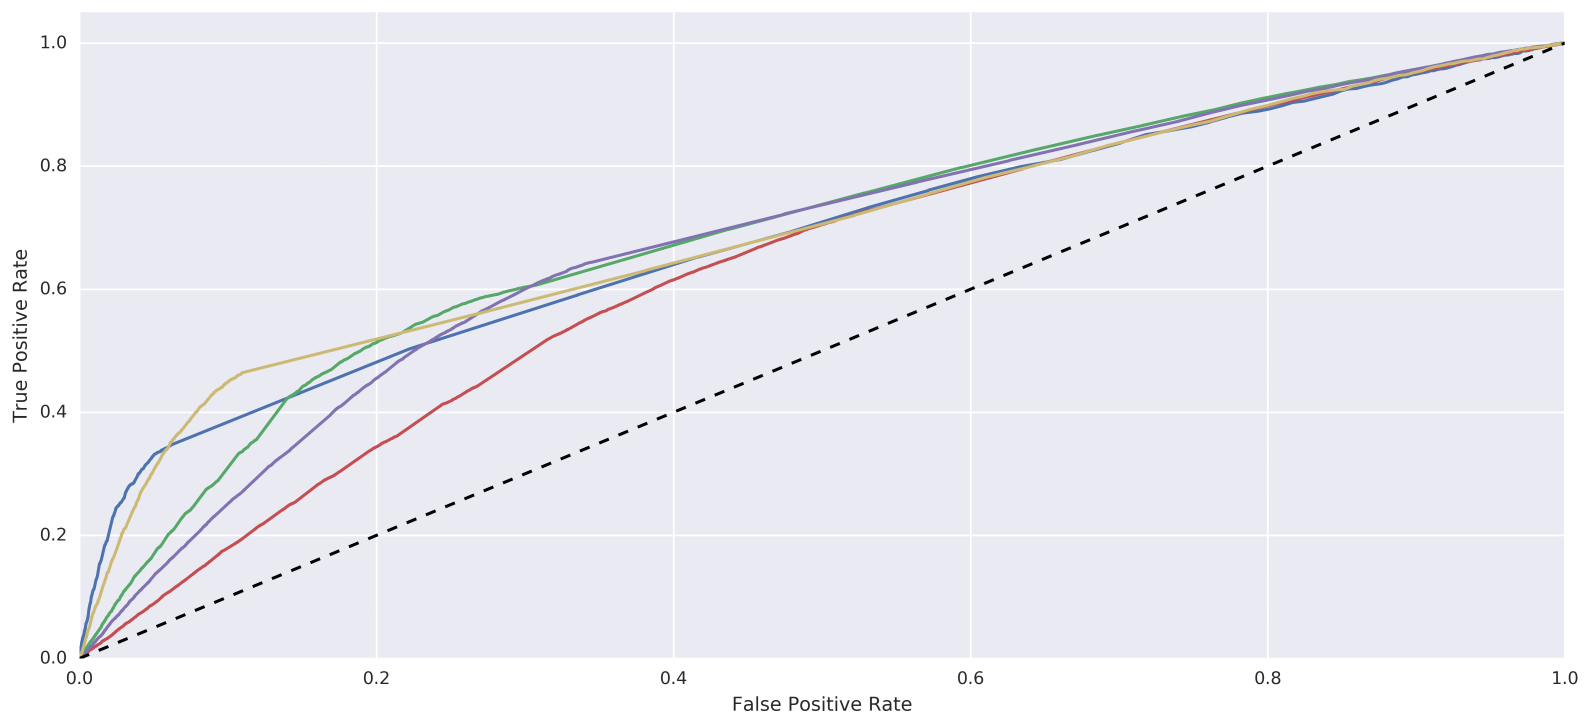
\includegraphics[width=\textwidth]{ROC_multiclass_wide.png}
		\caption{ROC Curves with \textit{False Positive Rates} plotted against the \textit{True Positive Rates}}
	\end{figure}
\end{frame}

\subsection{Next Steps}
\begin{frame}{Next Steps}
\note{%
	This paper presents a Bayesian approach to inferring the Socioeconomic Index of people according to the social graph based on a probabilistic hypothesis, but we can use several features of the graph, such as average call time to each category, to create a new algorithm for inferring this data.

	(pause)

	We also aren't using a big part of the dataset, which contains data for age and gender.

	(pause)

	We can locate the antenna of a small part of the voice calls. An obvious next step would be to add geographical location of the user to improve our inference.
}

\begin{itemize}
	\item<1-> Extending the work to multiple categories.
	\item<1-> A Machine Learning approach to the algorithm using more data from the social graph.
	\item<2-> Using more demographic data (age \& gender) to infer socioeconomic index.
	\item<3-> Make use of geographical location.
\end{itemize}
\end{frame}

\section{Bibliography}

\begin{frame}{Bibliography}

\renewcommand*{\bibfont}{\footnotesize}
\printbibliography{}

\end{frame}

\section{Questions}

\begin{frame}
	\Huge
	\begin{center}
	\begin{tabular}{@{}r@{}c@{}l@{}}
		&Questions&?\scalebox{.8}{?\scalebox{.8}{?\scalebox{.8}{?\scalebox{.8}{?\scalebox{.8}{?\scalebox{.8}{?}}}}}} \\
		&&\\
		\scalebox{.8}{\scalebox{.8}{\scalebox{.8}{\scalebox{.8}{\scalebox{.8}{\scalebox{.8}{?`}?`}?`}?`}?`}?`}?`&Preguntas&?\scalebox{.8}{?\scalebox{.8}{?\scalebox{.8}{?\scalebox{.8}{?\scalebox{.8}{?\scalebox{.8}{?}}}}}}
	\end{tabular}
	\end{center}
\end{frame}

\end{document}
